\chapter{Doppler Shift} \label{ch:Doppler}

Satellite RF signals are shifted in frequency proportionally to the line-of-sight velocity between the satellite and ground station, due to the Doppler effect. The Doppler frequency depends on time, on the location of the ground station, and on the orbit of the satellite, as well as on the carrier frequency \autocite{dopplergnuradio}. In satellite communications, it is common to correct for the Doppler present in the downlink signals before processing them. It is also common to correct for the uplink Doppler before transmitting an uplink signal, so that the satellite receiver sees a constant frequency.

\section{A Model for the LEO Satellite Doppler Shift} \label{sec:doppler_char}

In Low Earth Orbit (LEO) satellite communications, the kinematic dynamics between the spaceborne platform and the terrestrial station introduce a pronounced, time-varying frequency translation governed by the Doppler phenomenon. To characterize this effect without the computational burden of iterative numerical trajectory propagation, an elegant analytical framework can be derived by applying spherical trigonometry under valid orbital simplifications (see this article \autocite{ali1998doppler}). Assuming a circular orbit, the trajectory of the satellite during its short visibility window can be tightly approximated by a great-circle arc in the Earth-Centered Earth-Fixed (ECEF) reference frame. Furthermore, the tangential velocity magnitude in the ECF frame exhibits minor variations and is effectively approximated by the constant angular velocity at the peak latitude, defined as $\omega_{F} \approx \omega_{s} - \omega_{E} \cos i$, where $\omega_{s}$ denotes the inertial orbital angular velocity, $\omega_{E}$ represents the Earth's rotation rate, and $i$ is the orbital inclination.

    \begin{figure}[!ht]
        \centering
        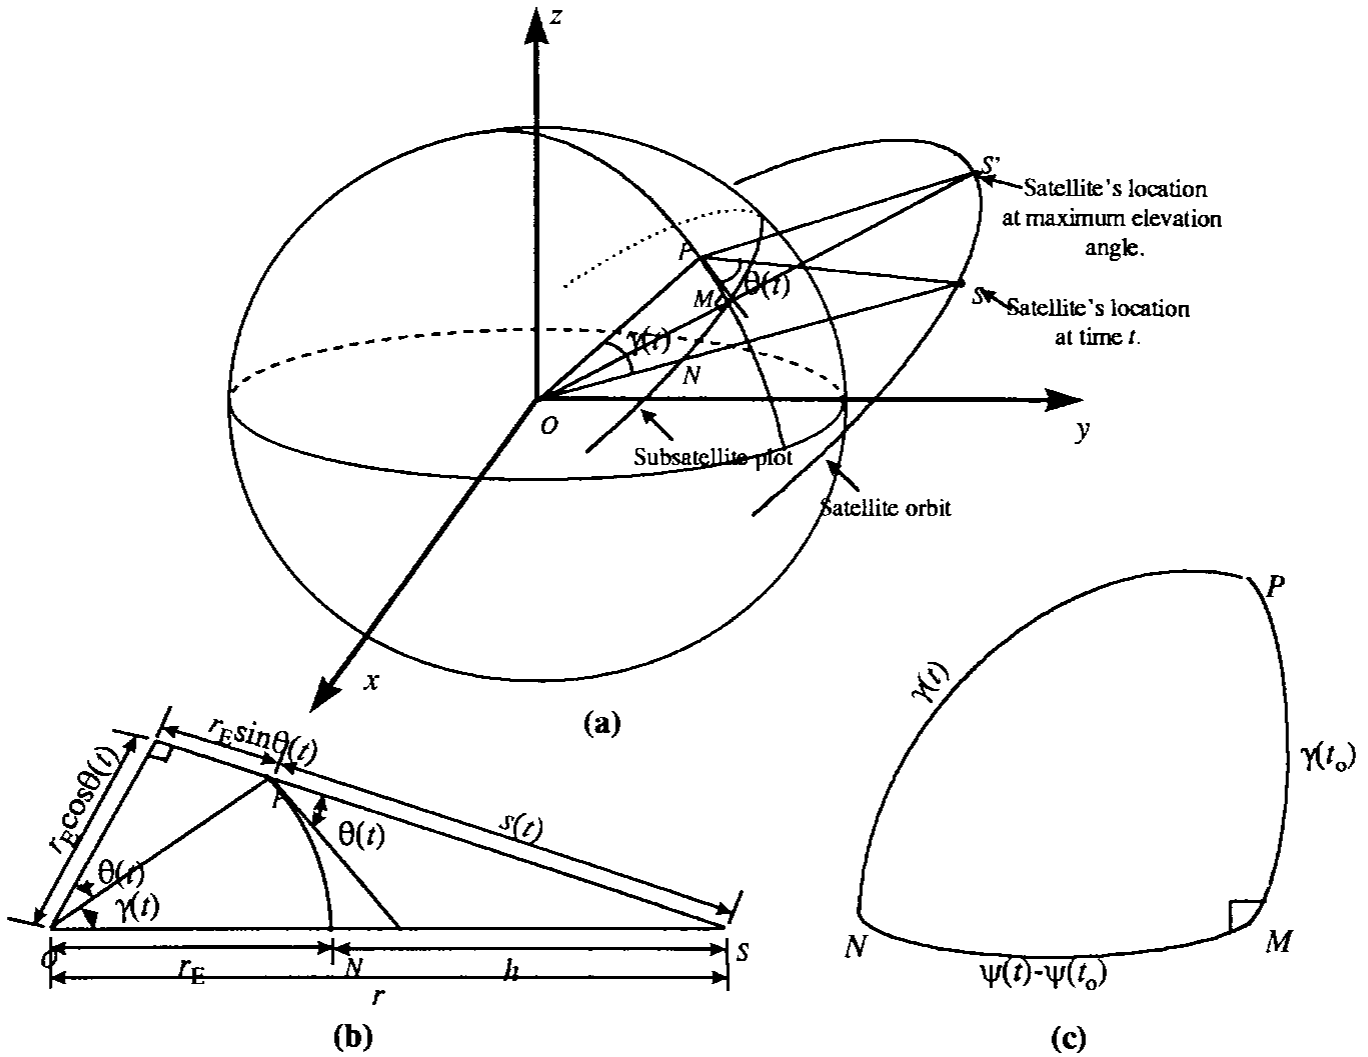
\includegraphics[width=0.65\textwidth]{figures/Inkscape/doppler_model.png} 
        \caption{Satellite geometry during visibility window at location P on earth. (a) Basic satellite geometry. (b) Plane triangle SOP . (c) Spherical triangle MNP. \autocite[Fig. 2]{ali1998doppler}}
        \label{fig:cc_diagram} 
    \end{figure}

By applying the law of cosines on the plane triangle formed by the Earth's center, the ground terminal, and the satellite's position, alongside the spherical cosine law for the projection of the ground trace, the dynamic slant range $s(t)$ and its time-derivative $\dot{s}(t)$ can be resolved analytically as a function of time $t$. Consequently, the normalized Doppler shift, formulated as $\frac{\Delta f(t)}{f_0} = -\frac{1}{c}\dot{s}(t)$, yields the following closed-form expression (Equation 5 in \autocite{ali1998doppler}):

\begin{equation}
\label{eq:doppler_model}
\frac{\Delta f(t)}{f_0} = -\frac{1}{c} \frac{r_{E}r \sin(\omega_{F} t) \cos \gamma_0 \cdot \omega_{F}}{\sqrt{r_{E}^{2}+r^{2}-2r_{E}r \cos(\omega_{F} t) \cos \gamma_0}}
\end{equation}

Within this analytical formulation, $f_0$ denotes the nominal downlink carrier frequency --- centered at $10.475$ GHz for the X-band system under analysis --- while $c$, $r_{E}$, and $r$ represent the speed of light, the mean radius of the Earth, and the orbital radius ($r = r_{E} + h$, where $h$ is the satellite altitude), respectively. The temporal variable $t$ is defined relative to the zero-Doppler instant ($t = 0$), which geometrically corresponds to the epoch of closest approach and maximum elevation. The constant angular distance $\gamma_0$ represents the central angle at the maximum elevation point, implicitly determined via the transcendental relation $\cos(\theta_{\max} + \gamma_0) = \frac{r_{E}}{r} \cos \theta_{\max}$, where $\theta_{\max}$ is the maximum elevation angle achieved during the specific pass. \Cref{eq:doppler_model} mathematically outlines a symmetric S-curve whose slope at the inflection point is explicitly parameterized by $\theta_{\max}$.


%%%%%%%%%%%%%%%%%%%%%%%%%%%%%%%%%%%%%%%%%%%%%%%%%%%%%%%%%%%%%%%%%%
\section{Two-Stage Doppler Compensation} \label{sec:doppler_comp}

As established by the analytical model, the macroscopic kinematic Doppler shift during an X-band pass can span hundreds of kilohertz. However, relying solely on an open-loop analytical model or orbital predictions is insufficient for maintaining a robust communication link. The combination of hardware oscillator drifts, Low Noise Block (LNB) offsets, and kinematic mismatches due to aging Two-Line Elements (TLEs) dictates that applying a perfectly inverted theoretical S-curve will never perfectly center the signal at baseband. A residual, time-varying Doppler shift will always persist.

To overcome this unpredictability and ensure continuous synchronization, our Software-Defined Radio (SDR) architecture implements a two-stage Doppler compensation strategy: a \textit{coarse} open-loop estimation followed by a \textit{fine} closed-loop tracking mechanism.

\begin{figure}[h]
    \centering
    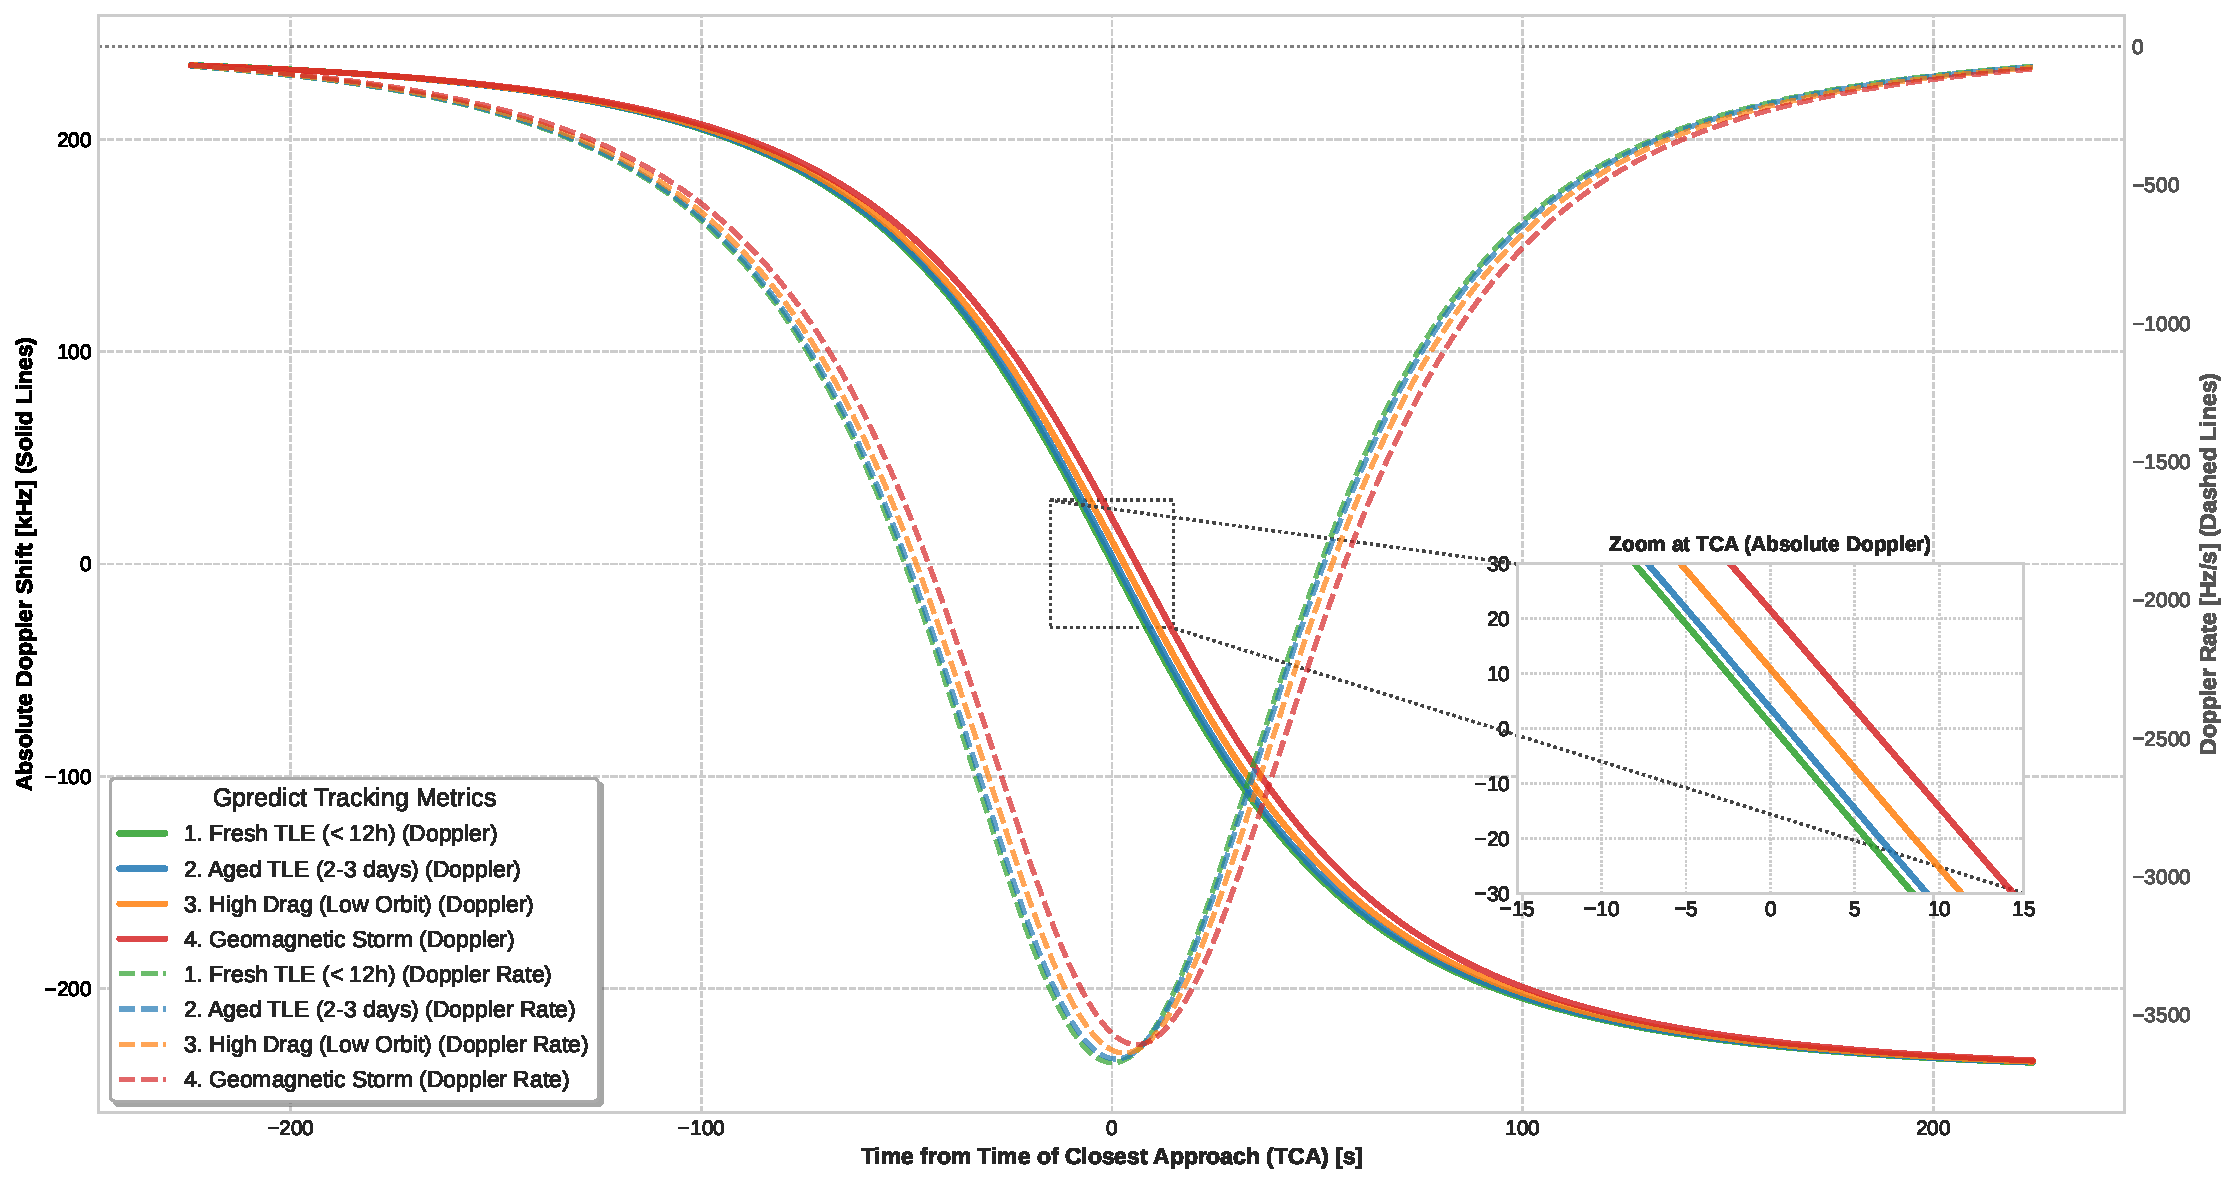
\includegraphics[width=1\textwidth]{figures/Inkscape/absolute_gpredict_doppler_curves.pdf}
    \caption{Doppler Curves \& Rates vs TLE Conditions.}
    \label{fig:doppler_curves}
\end{figure}

\subsection{Coarse Compensation via Orbital Prediction}
\label{subsec:coarse_comp}

The first stage involves removing the bulk of the predictable frequency shift. To achieve this, we rely on an open-loop coarse correction using Two-Line Elements (TLEs) to predict the satellite's altitude and position. A TLE set encodes the orbital elements of an Earth-orbiting object at a specific epoch. However, due to the limited number of decimals in the format and the underlying mathematical limitations of the SGP4 propagation model, even a freshly issued TLE possesses an inherent positional average error of approximately 3 kilometers \autocite{vallado2001fundamentals}. Because these ephemerides inevitably correspond to an orbit in the past compared to the true physical orbit at the time of reception, kinematic mismatches always arise.

To process these orbital parameters dynamically, we utilize Gpredict, a highly regarded open-source real-time satellite tracking and orbit prediction application. Gpredict \autocite{gr_gpredict_doppler} continuously calculates the expected Doppler shift using the SGP4 propagation model based on the freshest available TLEs and the ground station's geographical coordinates. While implementing an SGP4 orbital propagator natively within the GNU Radio flowgraph might initially seem more integrated, outsourcing this task to an external tool offers crucial architectural advantages. Specifically, it decouples the low-rate orbital mechanics calculations from the high-speed DSP pipeline. This separation ensures that the computational resources within the flowgraph are strictly dedicated to sustaining the high 25~Mbps real-time demodulation rate without risking buffer overflows.

Gpredict interfaces with the GNU Radio flowgraph via a network socket connection, targeting an XMLRPC Server block. As the satellite passes overhead, Gpredict acts as the master controller, periodically sending target frequency update commands to a local oscillator (Signal Source) or a frequency-shifting block inside GNU Radio. This dynamically shifts the incoming RF stream in the opposite direction of the predicted Doppler curve.

\subsection{Hardware Drifts and Residual Error Analysis}
\label{subsec:hardware_drifts}

While the coarse correction effectively removes the macroscopic Doppler shift, real-world links suffer from unpredictable hardware deviations that add up to the TLE kinematic mismatch. Both the satellite's transmitter and the receiver's Low Noise Block (LNB) introduce thermal and long-term frequency drifts. For example, LNB offsets can easily introduce several kilohertz of baseline error. To simulate these hardware effects accurately, the system parameters have been modeled taking as reference the official datasheets of said components \autocite{LNB_Manual}.

\begin{figure}[h]
    \centering
    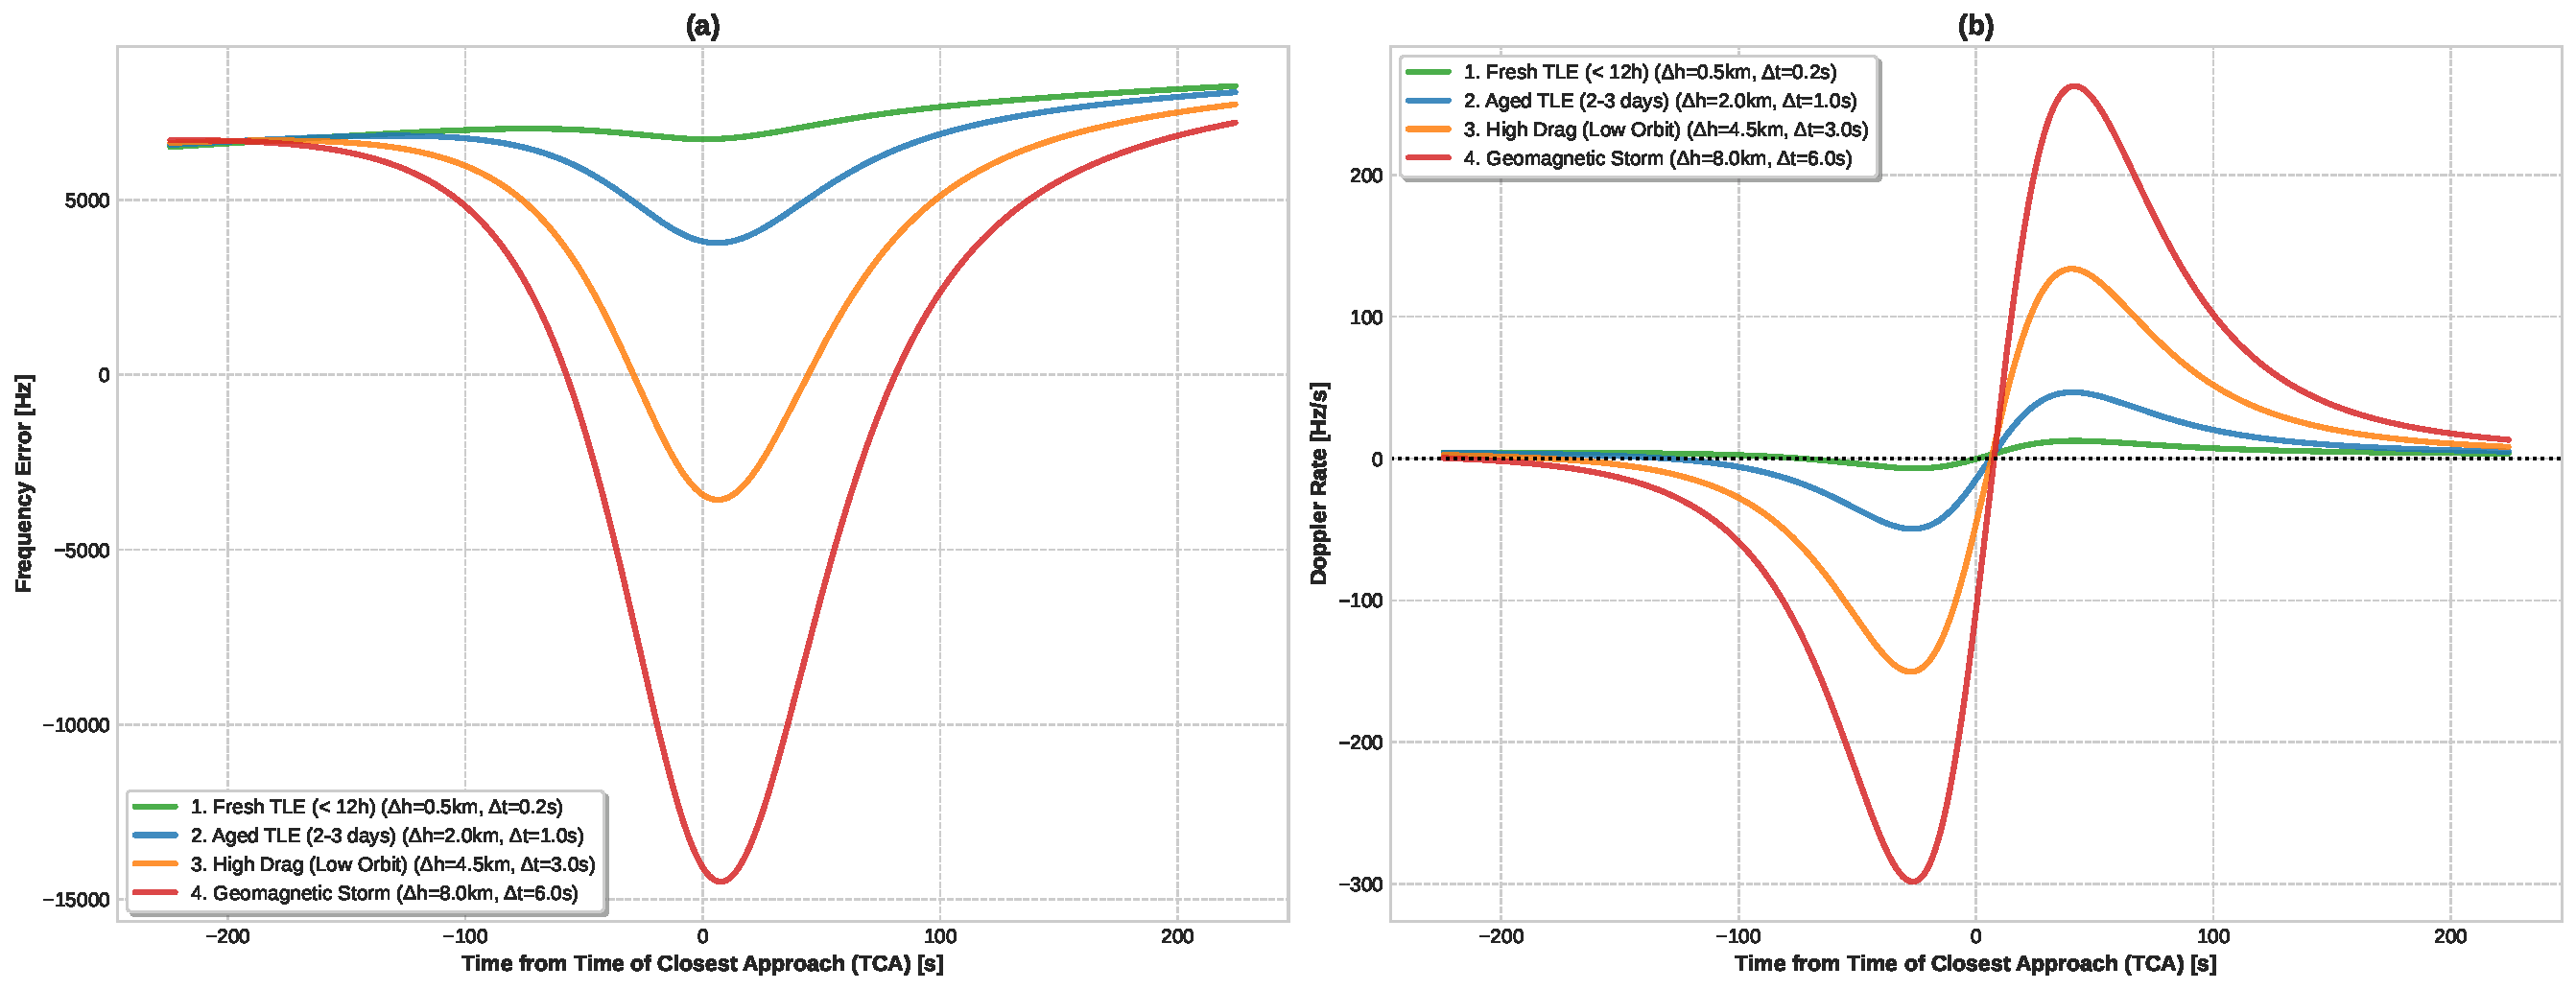
\includegraphics[width=1\textwidth]{figures/Inkscape/doppler_residuals_analysis.pdf}
    \caption{(a) Total Residual Error vs TLE Accuracy. (b) Derivative of Residual Error (Doppler Rate).}
    \label{fig:doppler_residuals}
\end{figure}

To fully characterize the system's robustness, several operational cases have been considered that represent different degrees of degradation in the orbital information, as illustrated in \Cref{fig:doppler_curves}. These simulated scenarios range from a nominal situation with recently updated TLEs (less than 12 hours old) to the standard degradation of the data after a couple of days. Furthermore, we model extreme situations such as high atmospheric friction or geomagnetic storms that induce delays of several seconds in the satellite's trajectory\footnote{For further context on these orbital perturbations, one can look at space weather reports \href{https://www.swpc.noaa.gov/impacts/satellite-drag}{\texttt{Space Weather Conditions NOAA}}, which discuss how events like geomagnetic storms increase atmospheric drag. A historical example is NASA's Solar Maximum Mission (SMM) spacecraft, which was reported to have "dropped as if it hit a brick wall" due to sudden atmospheric expansion.}. 

\begin{figure}[h]
    \centering
    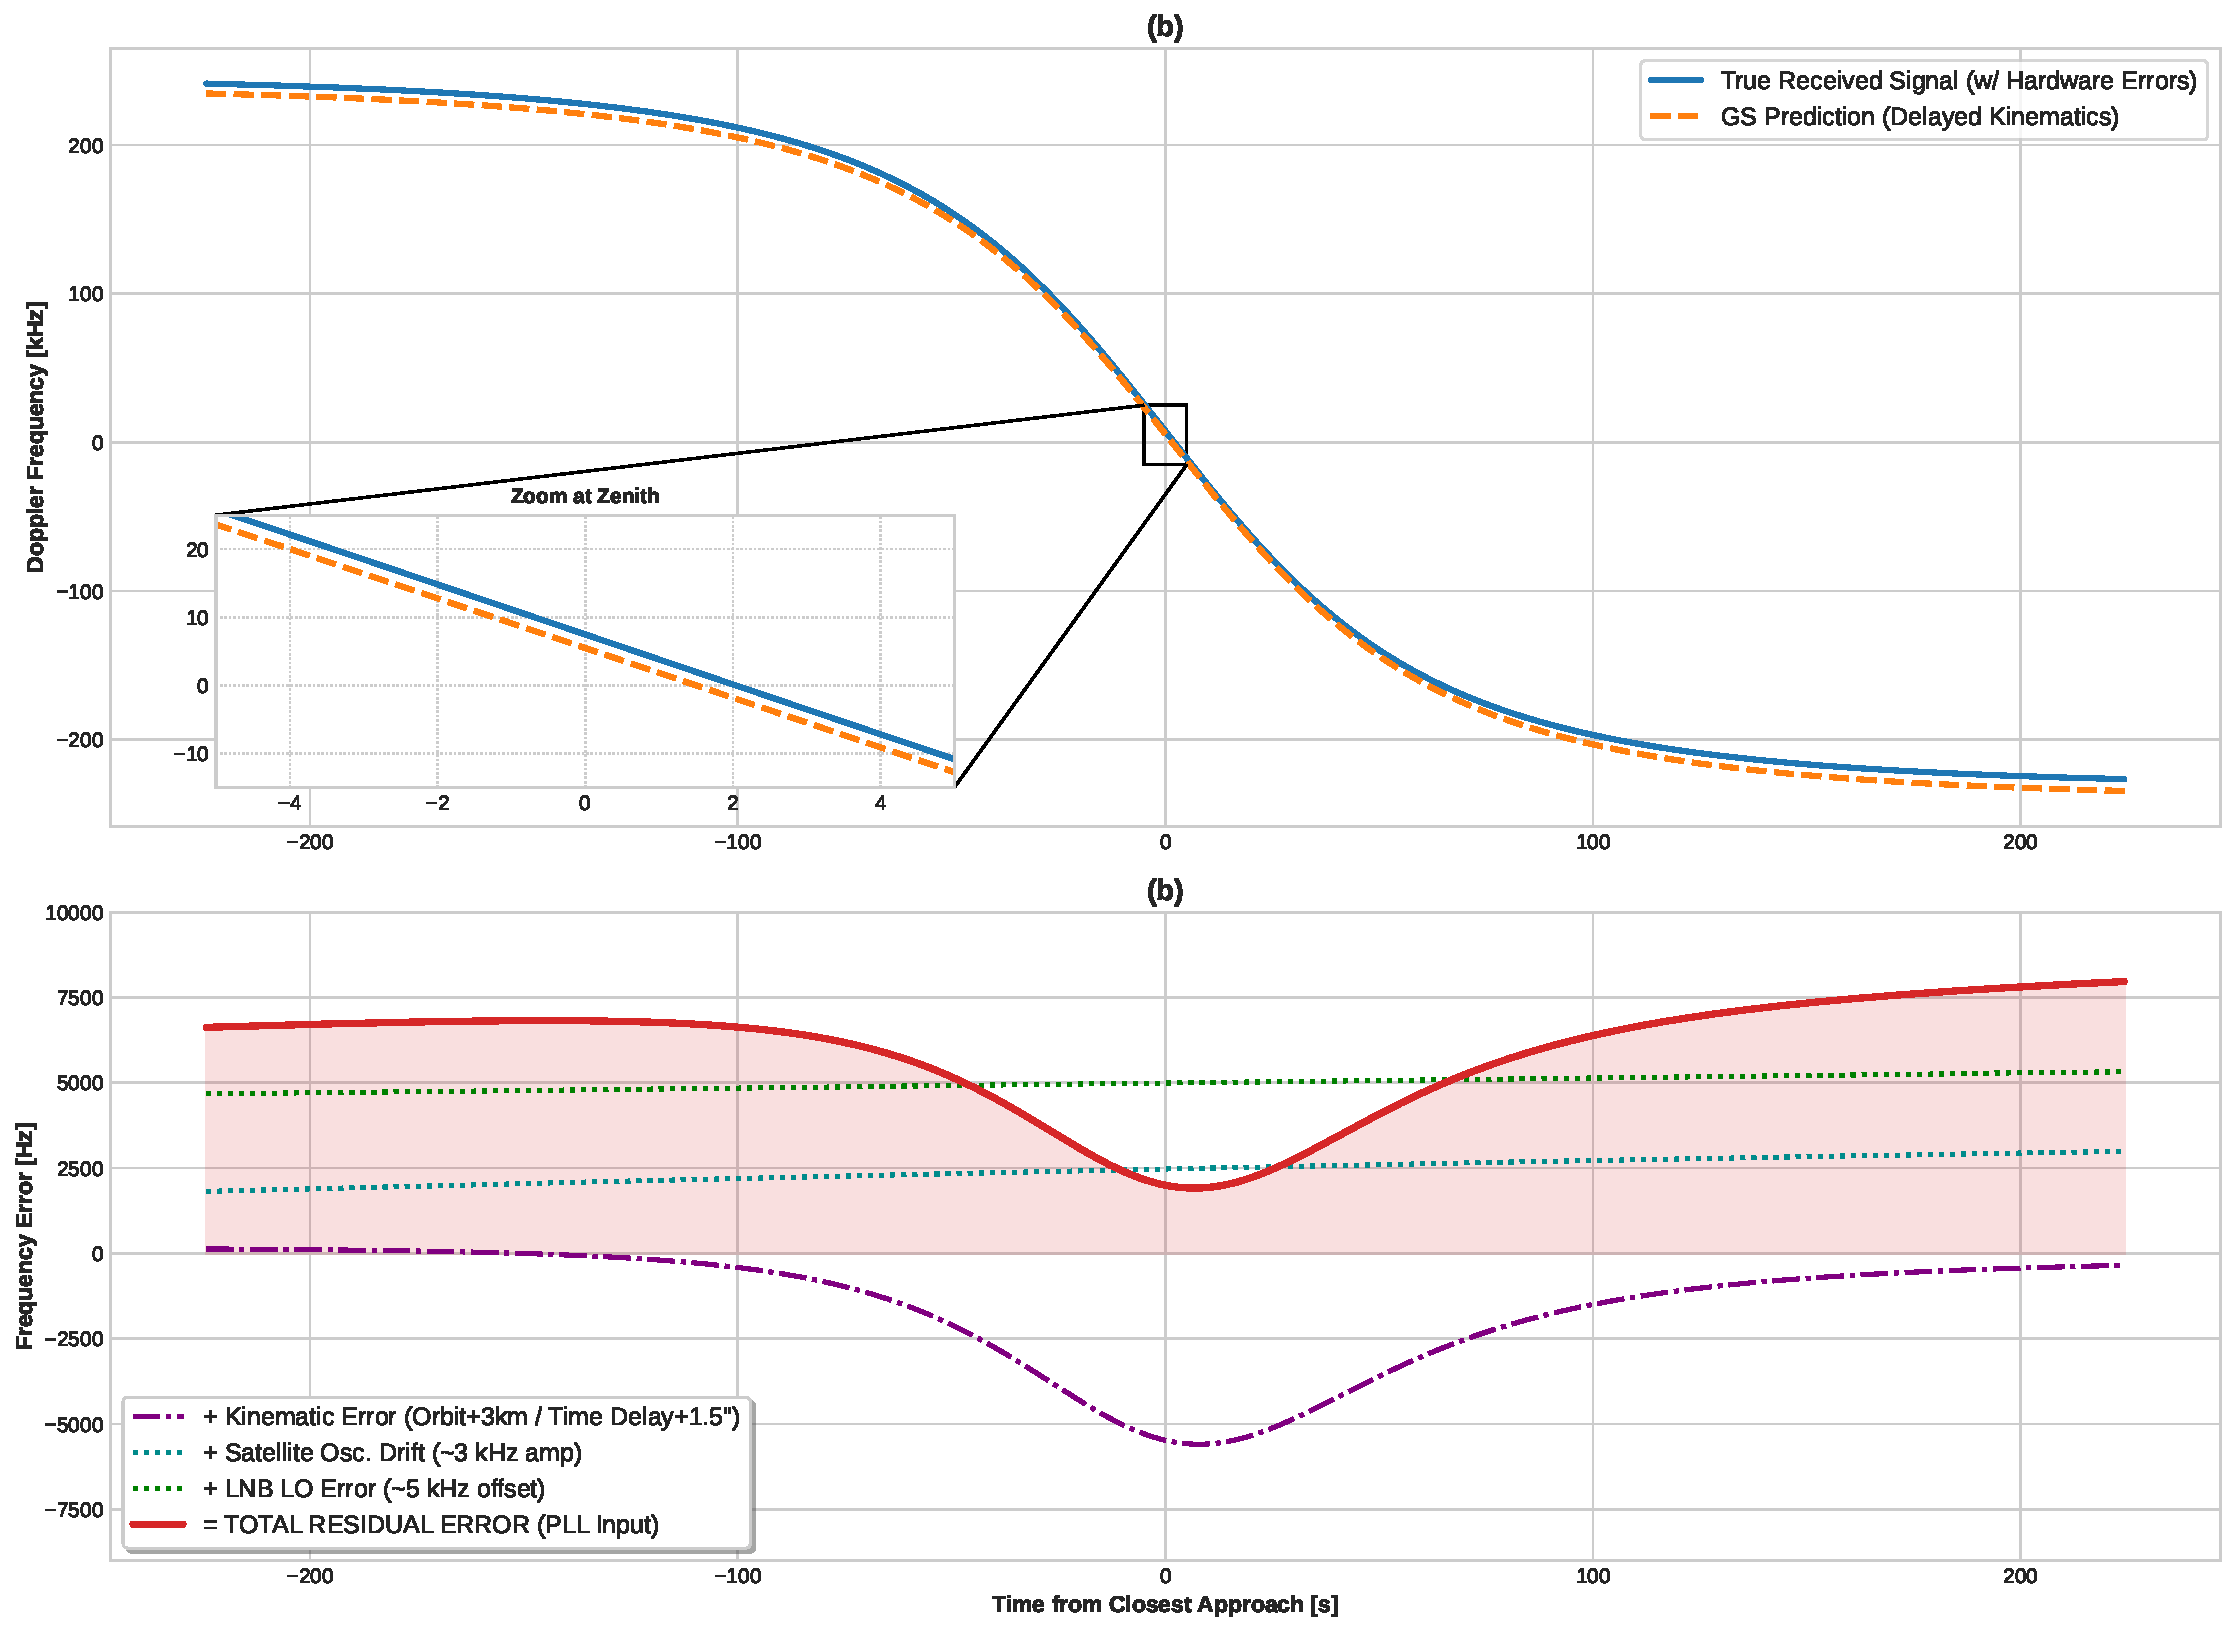
\includegraphics[width=1\textwidth]{figures/Inkscape/doppler_curve_case.pdf}
    \caption{A particular case of a Coarse Doppler Correction. (a) True vs Predicted Doppler. (b) Residual Error after coarse correction (What the Modem Actually Sees).}
    \label{fig:doppler_curve_case}
\end{figure}

These simulations allow us to deeply evaluate the impact of altitude and time deviations on the total frequency residual and the Doppler rate of change, which are critical parameters to guarantee receiver lock during the pass, as seen in \Cref{fig:doppler_residuals}. 

To visualize the practical outcome of this first stage, \Cref{fig:doppler_curve_case} illustrates a particular scenario of coarse Doppler correction. Part (a) plots the true received signal against the delayed kinematic prediction provided by Gpredict. Because the coarse stage relies on this imperfect prediction, it inherently leaves behind a dynamic residual frequency error. This leftover error, depicted in \Cref{fig:doppler_curve_case}(b), represents exactly what the software modem sees after the coarse compensation has been applied.


\subsection{Fine Frequency Tuning: The Costas Loop}
\label{subsec:fine_tuning_costas}

Because the coarse stage leaves behind this dynamic residual frequency error --- which fluctuates unpredictably over time due to the combination of TLE aging, SGP4 limitations, and hardware oscillator drifts --- a secondary tracking stage is strictly required to reliably demodulate the downlink. To finely tune the frequency, eliminate the residual offset shown in \Cref{fig:doppler_curve_case}(b), and guarantee phase lock during the pass, we introduce a second step: a discrete Costas loop designed to autonomously track and compensate for these residual fluctuations. This closed-loop estimation block will be addressed in detail in \Cref{sec:costas_loop}.
%%%%%%%%%%%%%%%%%%%%%%%%%%%%%%%%%%%%%%

\section{The Discrete Costas Loop} \label{sec:costas_loop}

In order to perform a fine frequency estimation, an element that tracks the frequency in real-time to correct it is necessary. Furthermore, this algorithm must be efficient since it will have to work with several million samples per second. Following a coherent demodulation architecture, the Costas Loop implemented in GNU Radio \href{https://wiki.gnuradio.org/index.php/Costas_Loop}{\texttt{Costas Loop Block}} represents effective solution to this problem. This block is well-established within the community and fully optimized for this function. The objective of this exposition is to provide a rigorous mathematical characterization of the entire block diagram, correlating each theoretical discrete-time equation directly with its corresponding C++ implementation. The mathematical representation of a phase-tracking loop and its subsequent simulations, as referenced in \Cref{fig:costas_loop}, will allow us to precisely deduce its behavior and performance as well as its stability.

    \begin{figure}[!ht]
        \centering
        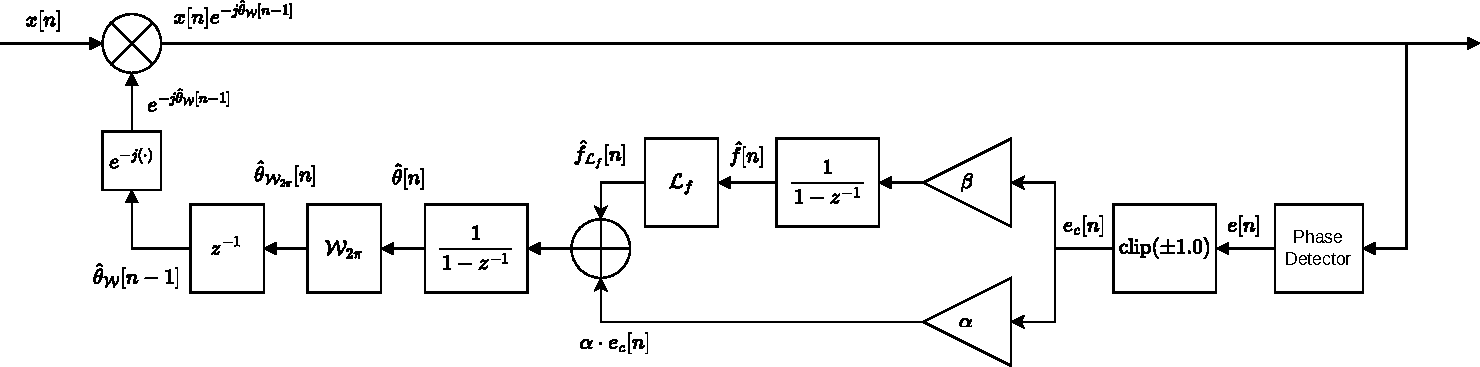
\includegraphics[width=1\textwidth]{figures/Inkscape/CostasLoop.drawio.pdf} 
        \caption{Diagram of the \href{https://wiki.gnuradio.org/index.php/Costas_Loop}{\texttt{Costas Loop Block}} coded by GNU Radio.}
        \label{fig:costas_loop} 
    \end{figure}

For each incoming discrete sample, the internal state vector $\bm{v}[k] = [\hat{f}[k], \hat{\theta}[k]]^T$ is updated according to the following state-space equation:

\begin{equation}
    \begin{bmatrix}
    \hat{f}[k+1] \\
    \hat{\theta}[k+1]
    \end{bmatrix}
    =
    \begin{bmatrix}
    \mathcal{L}_f & 0 \\
    0 & \mathcal{W}_{2\pi}
    \end{bmatrix}
    \left(
    \begin{bmatrix}
    1 & 0 \\
    1 & 1
    \end{bmatrix}
    \begin{bmatrix}
    \hat{f}[k] \\
    \hat{\theta}[k]
    \end{bmatrix}
    +
    \begin{bmatrix}
    \beta \\
    \alpha + \beta
    \end{bmatrix}
    \cdot e_c[k]
    \right)
\end{equation}

The Costas Loop implemented in GNU Radio consists of several key stages. First, the signal is rotated by the phase offset estimated in the previous stage. The phase detector obtains a new error metric to then begin the proportional-integral (PI) stage. Each stage is detailed now.

\subsection{Phase Derotation}

The signal flow commences with the discrete complex baseband input signal $x[n]$, which arrives at the receiver carrying an instantaneous phase perturbation. The primary operational stage of the diagram involves a complex multiplier (or mixer) that interacts the input signal with the corrective feedback phasor generated by the Numerically Controlled Oscillator (NCO). 
\begin{cpp}
const gr_complex nco_out = gr_expj(-d_phase);
gr::fast_cc_multiply(optr[i], iptr[i], nco_out);
\end{cpp}

\vspace{-2.25mm}
Consequently, the phase-corrected output signal $y[n]$ is defined by the discrete equation:
$$y[n] = x[n] \cdot e^{-j\theta[n-1]}$$
This operation rotates the sample according to the estimated phase deviation.

\subsection{Nonlinear Phase Detection and Error Metric Extraction} \label{subsec:phase_detection}
Following the derotation, the corrected complex sequence $y[n] = \Re\{y[n]\} + j\Im\{y[n]\}$ is passed to the Phase Detector (PD) block, whose mathematical objective is to suppress the underlying data modulation and isolate the scalar angular deviation.
\begin{cpp}
return ((sample.real() > 0.0f ? 1.0f : -1.0f) * sample.imag() -
        (sample.imag() > 0.0f ? 1.0f : -1.0f) * sample.real());
\end{cpp} \vspace{-2.25mm}

The result will be proportional to the sine of the phase difference between the vectors, providing a linear error metric for small angular deviations:

\begin{equation} \label{eq:error_metric}
    e[n] = \text{sgn}(\Re\{y[n]\}) \cdot \Im\{y[n]\} - \text{sgn}(\Im\{y[n]\}) \cdot \Re\{y[n]\}
\end{equation}

On the other hand, under conditions where the receiver can estimate the signal-to-noise ratio (\(\mathsf{SNR}\)), the algorithm transitions towards a $\mathsf{Maximum}$ $\mathsf{Likelihood}$ (\(\mathtt{ML}\)) estimator over $\mathsf{AWGN}$ channels. In this regime, the sign operator is replaced by a hyperbolic tangent scaled by the instantaneous noise parameter $\gamma$:
\begin{equation} \label{eq:ml_estimator}
    e[k] = \tanh(\gamma \cdot I_{out}[k]) \cdot Q_{out}[k] - \tanh(\gamma \cdot Q_{out}[k]) \cdot I_{out}[k]
\end{equation}
At low \(\mathsf{SNR}\) ($\gamma \ll 1$), the Taylor approximation $\tanh(x) \approx x$ asymptotically reduces the discriminator to a classic fourth-power Costas loop, avoiding the amplification of thermal noise that a rigid hard-limiter would cause.

Furthermore, the algorithm imposes a strict symmetric hard-limiter on the error signal and keeps it strictly within the interval $[-1.0, 1.0]$.
\begin{cpp}
    d_error = gr::branchless_clip(d_error, 1.0);
\end{cpp}\vspace{-2.25mm}

\subsection{The Loop Filter}

The bounded scalar error signal $e[n]$ is subsequently split into the parallel proportional and integral branches (PI filter) of the digital loop filter. This filter dictates the dynamic trajectory of the system by updating two internal state variables: the frequency estimate $f[n]$ and the phase estimate $\theta[n]$. The discrete-time difference equations governing this dynamic core are:
\begin{align}
    \hat{f}[k+1] &= \hat{f}[k] + \beta \cdot e_c[k] \label{eq:integral_branch} \\
    \hat{\theta}[k+1] &= \hat{\theta}[k] + \hat{f}[k+1] + \alpha \cdot e_c[k] \label{eq:prop_branch}
\end{align}
where $\alpha$ and $\beta$ are the proportional and accumulative gains, respectively.
\begin{cpp}
void advance_loop(float error)
{
    d_freq = d_freq + d_beta * error;
    d_phase = d_phase + d_freq + d_alpha * error;
}
\end{cpp}\vspace{-2.25mm}

The complete transfer function from the phase error $E(z)$ to the NCO phase $\Phi_{nco}(z)$ (see \Cref{fig:costas_loop}) is:
\begin{equation} \label{eq:transfer_function}
    H_{loop}(z) = \frac{\Phi_{nco}(z)}{E(z)} = \underbrace{z^{-1}}_{\text{NCO Delay}} \cdot \underbrace{\frac{1}{1-z^{-1}}}_{\text{Phase Accum.}} \left( \alpha + \beta \cdot \underbrace{\frac{1}{1-z^{-1}}}_{\text{Freq. Accum.}} \right)
\end{equation}
The aforementioned gains are calculated from the transfer function in the analog domain. PLL theory defines two key variables: the damping factor ---which is fixed at $\sqrt{2}/2$--- and the bandwidth ---the only configurable parameter---. To transition to the digital domain, a bilinear transform is performed to ensure the stability of the system. Then, the values of the parameters $\beta$ and $\alpha$ are calculated as follows:
\begin{align}
    \alpha &= \frac{4\zeta B_{n}}{1 + 2\zeta B_{n} + B_{n}^2} \label{eq:alpha} \\
    \beta &= \frac{4B_{n}^2}{1 + 2\zeta B_{n} + B_{n}^2} \label{eq:beta}
\end{align}
For further details on the analog to digital domain and development of \Cref{eq:beta} and \Cref{eq:alpha}, refer to \autocite[Chapters 2 \& 13]{gardner2005}.





\section{Costas Loop Characterization}

Once the mathematical model of the Costas Loop implemented in GNU Radio has been characterized, we will demonstrate its operational behavior through simulations. Understanding the algorithm's performance boundaries in a practical scenario is crucial for properly configuring its parameters and delivering a functional solution. 

As previously discussed, the loop must fulfill at least two key functions. First, it requires an acquisition range compatible with the scenarios proposed in \Cref{fig:doppler_residuals}. Second, given that the frequency varies rapidly over time --- especially during the time of closest approach --- the loop must be capable of tracking this frequency dynamically to maintain lock. To verify these requirements, we have conducted three experiments analyzing the following characteristics.

\subsection{Experiment 1: Transient Response}

To evaluate the loop's transient response, \Cref{fig:costas_plot} plots the step response of the system when subjected to an instantaneous 10 kHz frequency deviation. The convergence time depends directly on the configured loop bandwidth. A wider bandwidth allows the loop to react more aggressively to phase errors, significantly reducing the acquisition time for higher values of $B_n$.

Furthermore, the transient response time must be sufficiently brief to continuously track the maximum Doppler rate of 300 Hz/s (further analyzed in \Cref{subsec:experiment_3}). By selecting an appropriate bandwidth, and considering that frames have a length of 1115 bytes --- assuming $I=5$ ---, this acquisition transition spans only a few tens to hundreds of bits. While a lack of synchronization over this duration might initially appear detrimental, it does not pose a significant operational issue for the overall link. This brief acquisition phase occurs exclusively during the initial signal lock-on period prior to data payload extraction. Any transient bit errors generated during this window are either absorbed by the Access Sync Marker (ASM) correlation search or inherently corrected by the concatenated FEC decoders once steady-state tracking is achieved. Moreover, in actual operation, the receiver tracks continuous kinematic curves rather than discontinuous 10 kHz steps, as previously illustrated in \Cref{fig:doppler_curve_case}.

\begin{figure}[h]
    \centering
    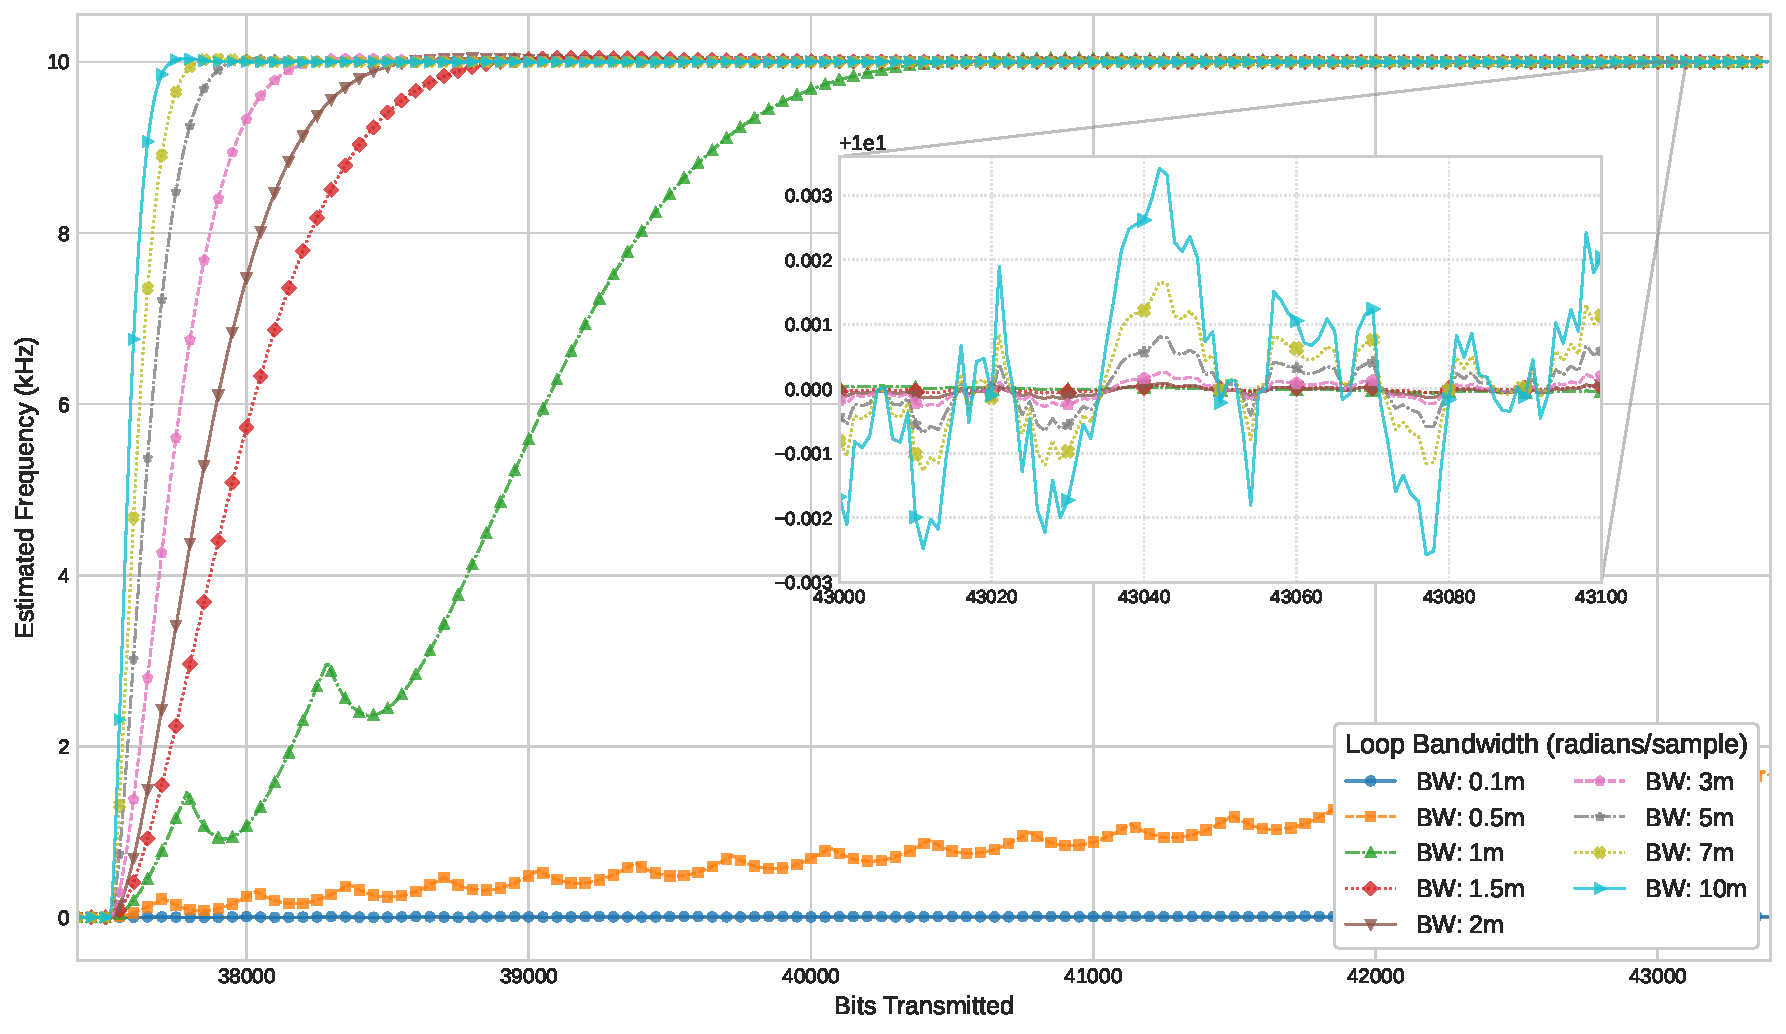
\includegraphics[width=1\textwidth]{figures/Inkscape/costas_loop_plot.pdf}
    \caption{Costas Loop frequency error transient response to a 10 kHz step across varying loop bandwidths.}
    \label{fig:costas_plot}
\end{figure}

\subsection{Experiment 2: Frequency Acquisition Range}

In digital receiver design, it is established in the literature that a pure Costas Loop typically loses lock when the initial frequency offset approaches approximately 5\% of the symbol rate \autocite{gardner2005}. Given the system's transmission rate of 12.5 Mbaud, the algorithm is theoretically constrained to a maximum frequency offset of around 0.625 MHz. This fundamental limitation is strictly corroborated by our empirical simulations and is largely independent of the configured loop bandwidth.

Recall \Cref{subsec:phase_detection}, which details the phase detector mechanism. When the residual frequency error is large enough that the phase rotation between consecutive samples exceeds the detector's decision boundary (for instance, $\pm 45^\circ$ in QPSK), ambiguity or aliasing occurs within the constellation. The received symbol crosses into an adjacent quadrant, misleading the decision-directed phase detector algorithm. The detector assumes an incorrect target symbol and consequently calculates an error metric with an inverted sign. As a result, the feedback loop instructs the NCO to correct in the diametrically opposite direction, pushing the system further away from the true carrier frequency. This immediately triggers a cycle slip and results in a total loss of synchronization.

\subsection{Experiment 3: Frequency Tracking} \label{subsec:experiment_3}

Finally, the Costas Loop must be capable of tracking a frequency transition of at least 300 Hz/s, as established in \Cref{fig:doppler_residuals}. To evaluate this, an oscillatory perturbation is introduced to simulate a dynamic frequency offset. As depicted in \Cref{fig:costas_perturbation}, the frequency shifts linearly (refer to the lower subplot displaying the derivative), allowing us to identify the exact point at which the loop loses lock.

\begin{figure}[h]
    \centering
    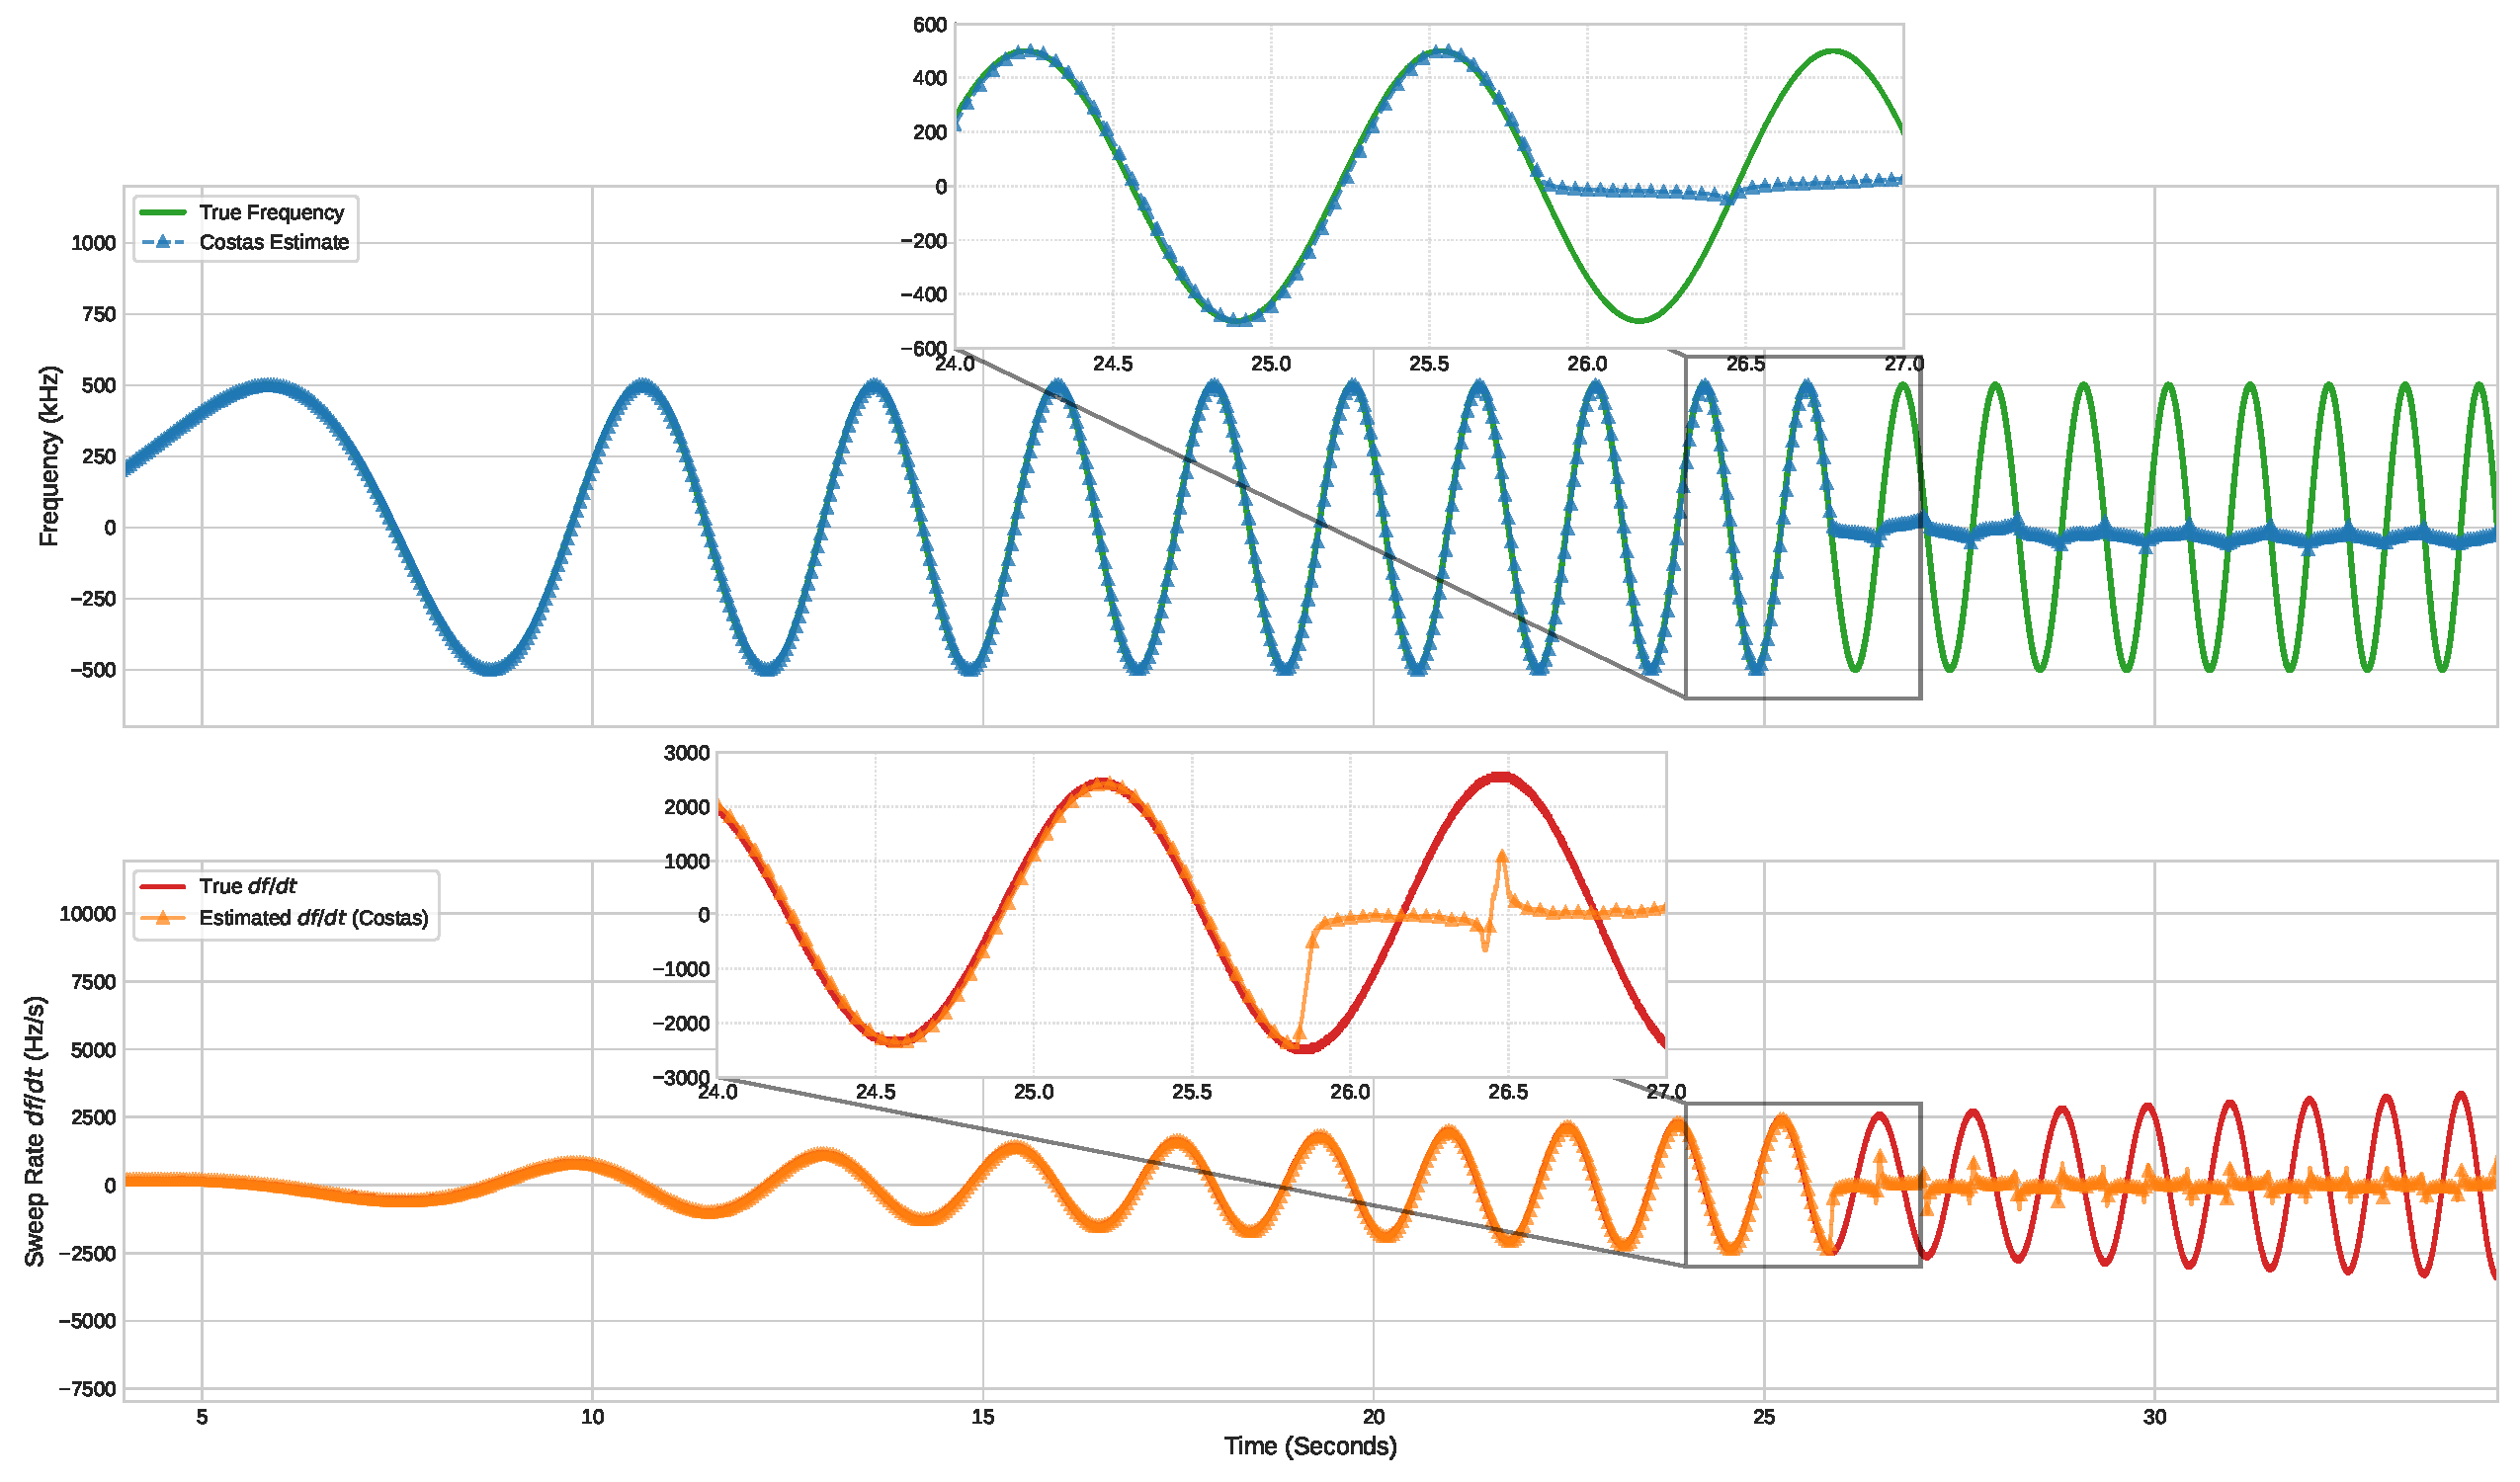
\includegraphics[width=1\textwidth]{figures/Inkscape/costas_vs_perturbation_zoom.pdf}
    \caption{Frequency tracking performance: True vs. Estimated frequency. The Costas Loop loses lock at a sweep rate of 2.5 kHz/s for a simulated loop bandwidth of $B_n = 5 \text{ mrad/s}$.}
    \label{fig:costas_perturbation}
\end{figure}

Consequently, evaluating this behavior across different bandwidths yields the experimental results shown in \Cref{fig:costas_robustn}. This figure is highly valuable as it enables the precise selection of the required bandwidth $B_n$ to configure the Costas Loop. According to the theoretical tracking limits defined by \autocite{gardner2005}, the maximum sweep rate that can be tracked is $\Delta\dot{\omega} \approx \omega_n^2 / 2$, which closely matches our empirical findings. This demonstrates that if our system must track a maximum drift of 300 Hz/s (see \Cref{fig:doppler_residuals}), we need to configure a loop bandwidth of at least $\approx 2 \text{ mrad/s}$. This establishes our stability region.

\begin{figure}[h]
    \centering
    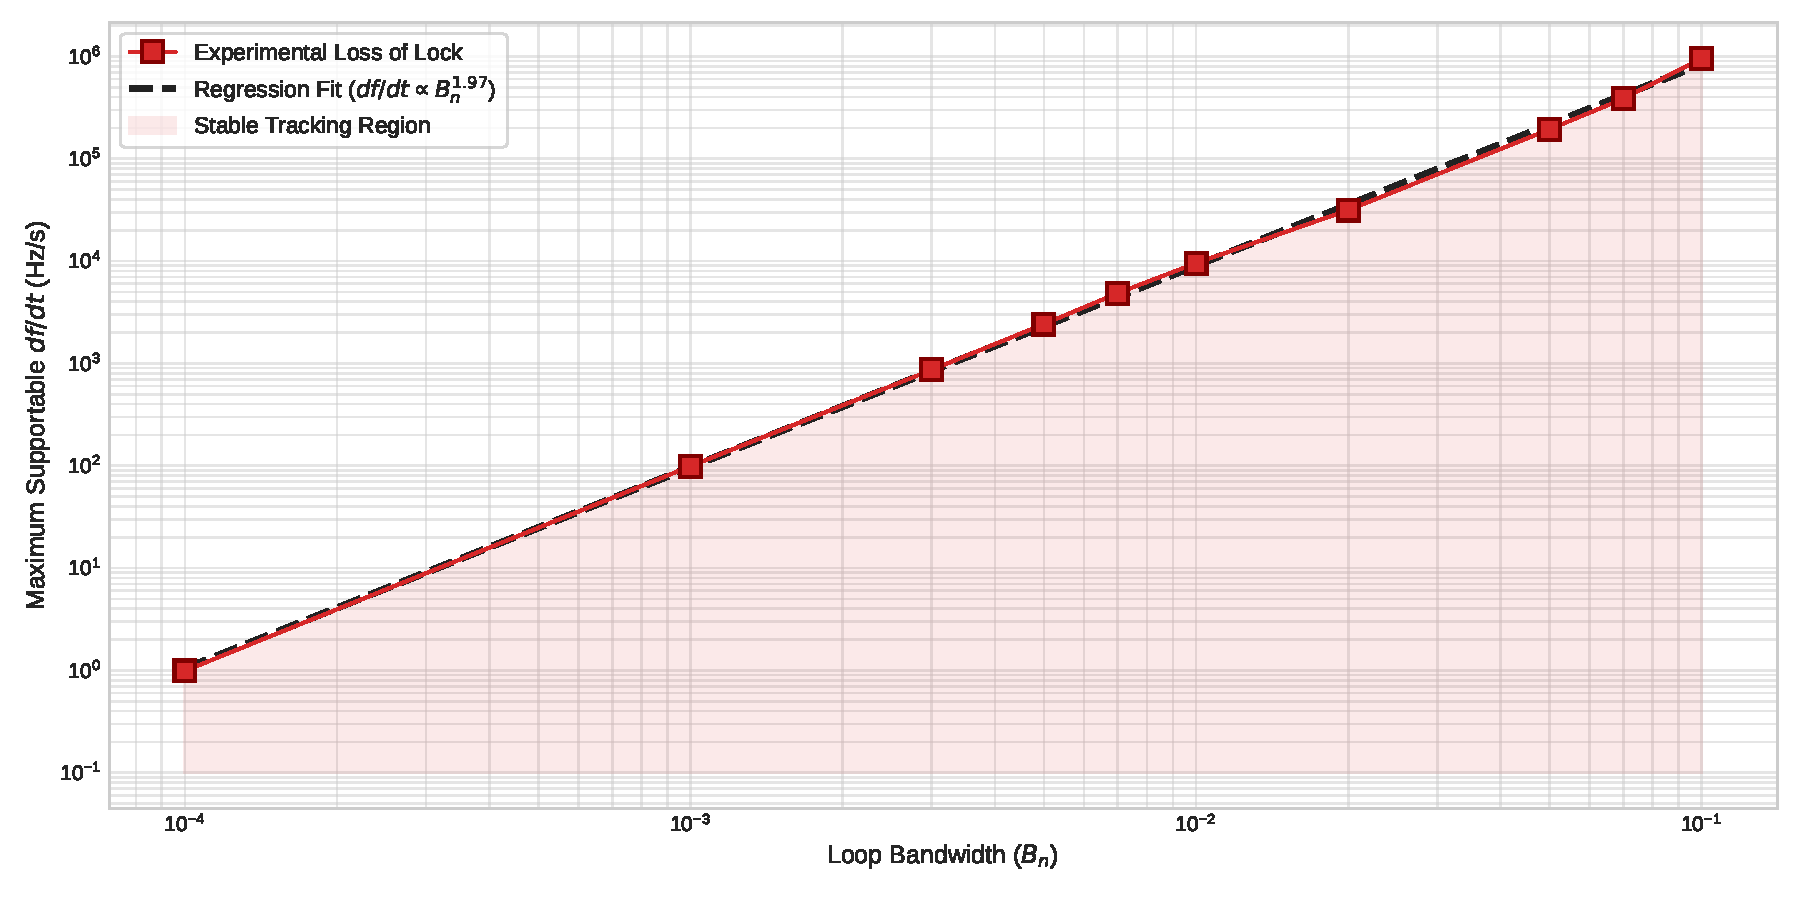
\includegraphics[width=1\textwidth]{figures/Inkscape/costas_robustness_analysis.pdf}
    \caption{Costas Loop Robustness: Maximum trackable frequency sweep rate ($df/dt$) versus Loop Bandwidth.}
    \label{fig:costas_robustn}
\end{figure}

Returning to \Cref{fig:costas_plot}, an examination of the magnified plot reveals that the frequency estimation exhibits oscillations that become more pronounced with wider configured bandwidths. There is a steep penalty for exceeding the optimal bandwidth, as extensively discussed in \autocite[Chapter 6]{gardner2005}. Specifically, the relationship between the loop bandwidth and the phase variance of the NCO is governed by the equation:
\begin{equation}
    \sigma_{\theta_{no}}^2 = \frac{2 N_0 B_L}{V_s^2} = \frac{W_0 B_L}{P_s} \text{ [rad}^2\text{]}
\end{equation}


The noise generated by the estimation process is superposed onto the data signal, causing a considerable degradation in link performance. This is clearly observed in \Cref{fig:BER_curves_Bn}. Because deviating from the optimal normalized bandwidth incurs a heavy cost, we recommend a value of at least 1 to 2 mrad/s to ensure the proper functioning of the link. According to the referenced figure, this operating point corresponds to the cyan curve.

\begin{figure}[!ht]
    \centering
    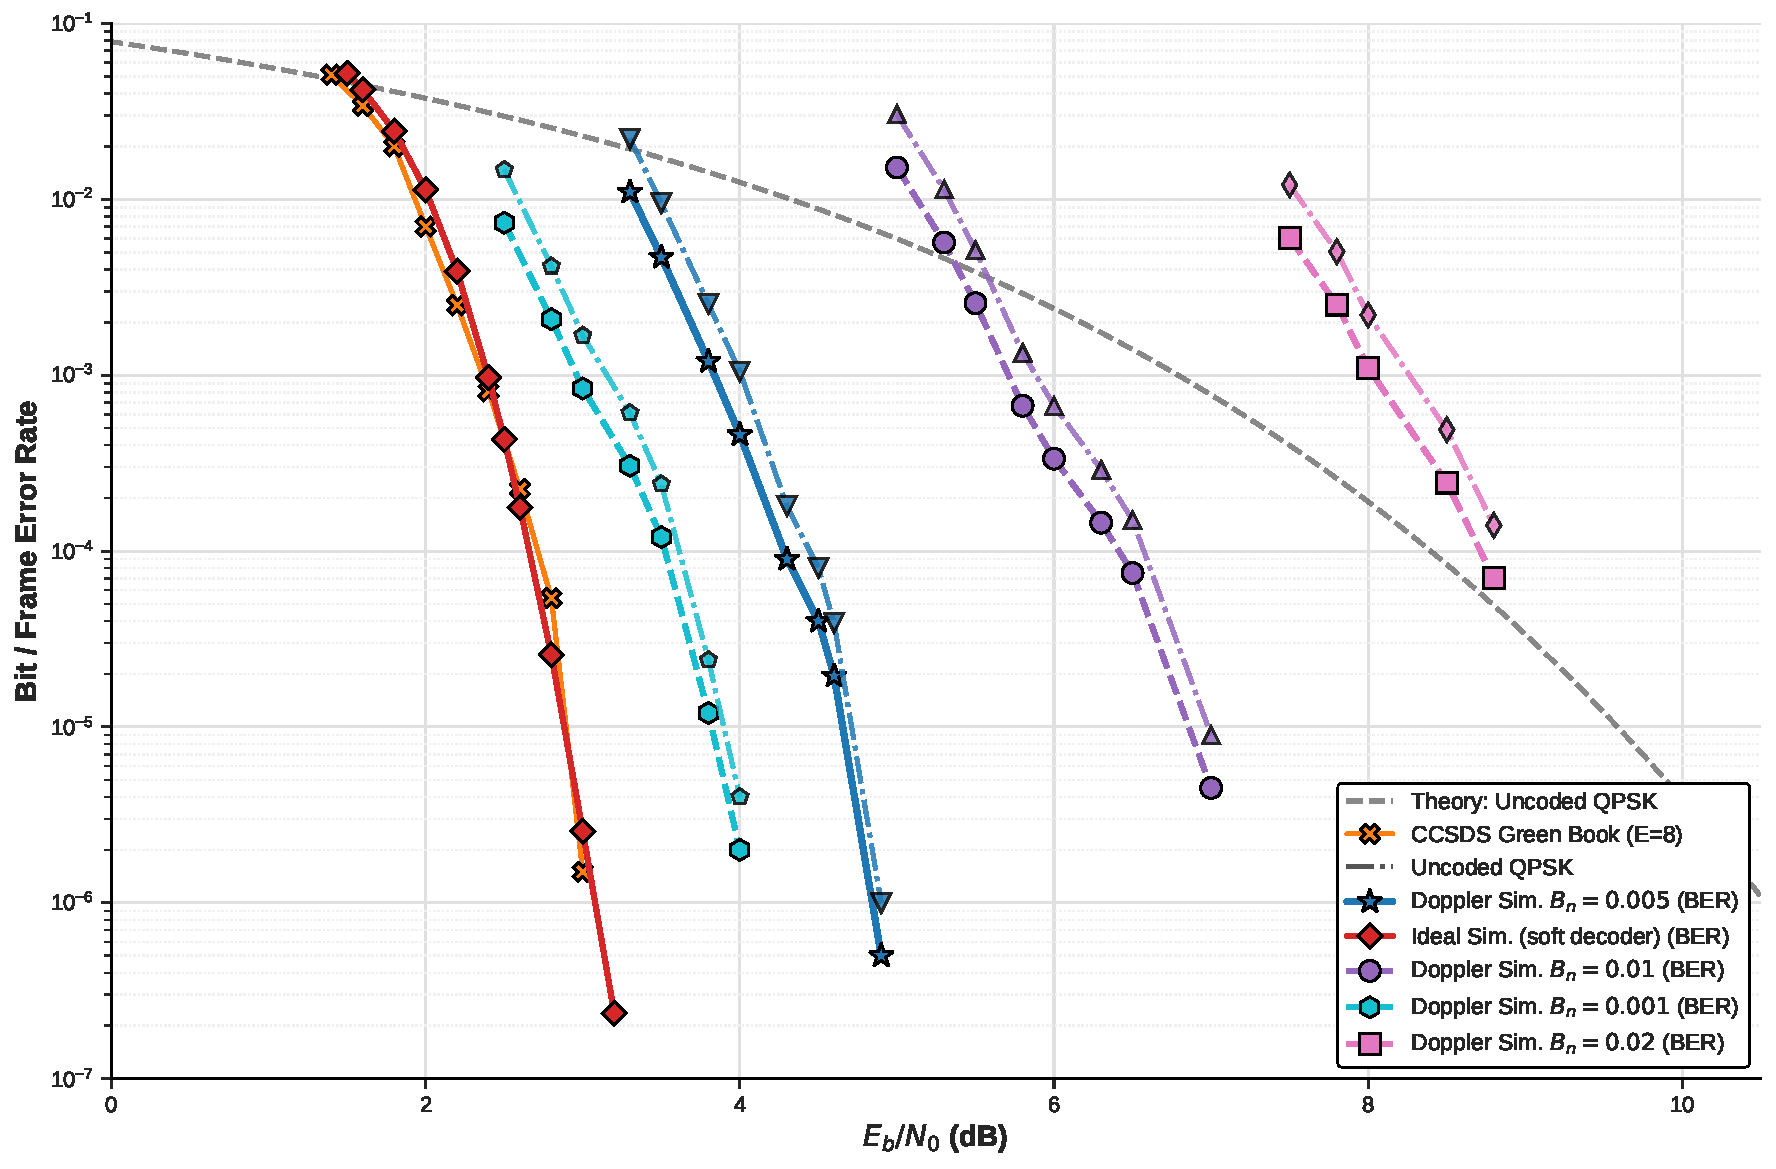
\includegraphics[width=1\textwidth]{figures/Inkscape/BER_curves_Bn.pdf}
    \caption{Comparative Bit Error Rate (BER) performance across different normalized loop bandwidths ($B_n$).}
    \label{fig:BER_curves_Bn}
\end{figure}
  
It must be noted that initial system simulations under these bandwidth configurations exhibited a higher than expected Frame Error Rate (FER), resulting in a significant number of dropped frames, as represented by the baseline pink curve shown in \Cref{fig:BER_curves_frame_sync}. This severe performance degradation is not a failure of the Costas Loop's tracking ability, but rather a fundamental consequence of unhandled phase ambiguities. While the loop successfully recovers the carrier frequency and achieves phase lock, decision-directed algorithms inherently exhibit an $N$-fold phase ambiguity (e.g., $90^\circ$ phase rotations in QPSK). If the loop locks onto an incorrect constellation quadrant, the demodulated bitstream is systematically inverted or rotated, rendering the data completely undecodable by the subsequent Forward Error Correction (FEC) blocks. To recover the true theoretical BER performance, the system requires a mechanism to resolve this ambiguity and detect the exact boundaries of the data structures. This critical requirement, and its specific algorithmic implementation, are addressed in the following chapter regarding Frame Synchronization (\Cref{ch:Frame_sync}).






